\documentclass[UTF8]{ctexart}
\usepackage{graphicx}
\usepackage{amsmath}
\usepackage{diagbox}
\usepackage{float}
\usepackage{listings}
\usepackage{url}
\usepackage{xcolor}
\newcommand{\tabincell}[2]{\begin{tabular}{@{}#1@{}}#2\end{tabular}}
\newcommand{\enabstractname}{Abstract}
\newenvironment{enabstract}{%
    \par\small
    \noindent\mbox{}\hfill{\bfseries \enabstractname}\hfill\mbox{}\par
    \vskip 2.5ex}{\par\vskip 2.5ex}  
\title{基于RaspberryPi的厕所空气质量智能在线监管系统}
\author{
陈彦宁
\ \ 刘涵之
\ \ 冯驰
\ \ 陈毓仁
\ \ 罗景致\\
\\指导教师:李磊
}

\date{上海交通大学\\2019 年 12月 13 日}
\begin{document}
\maketitle\pagebreak
\begin{abstract}
\addcontentsline{toc}{section}{摘要}
本课题通过研究厕所管理方案,设计开发了一种基于RaspberryPi的厕所空气质量智能在线监管系统。此套系统可适用于大规模的(公共)厕所臭味情况监控与除臭管理,为现实生活中需要大规模管理厕所的情况提供了智能的解决方案,在很大程度上降低了大规模厕所维护的人力成本。本系统在开发时将核心代码进行了深度封装,为在现实生活中的部署提供了很大的便利。

\centering
本系统的演示版本 : \url{https://brownsense.misaka.center/}

本系统的开源地址 : \url{https://github.com/PhotonQuantum/BrownSense}

	\centering
    \textbf{关键词:} 物联网, WEB, 厕所空气质量
\end{abstract}

\begin{enabstract}
This subject has developed a smart online monitoring system for toilet air quality based on RaspberryPi by studying toilet management schemes. This system can be applied to large-scale toilet odor situation monitoring and deodorization management. It provides intelligent solutions for situations that require large-scale toilet management in real life, and greatly reduces manpower for large-scale toilet maintenance cost. The core code was deeply encapsulated during the development of this system, which provided great convenience for deployment in real life.

\centering
Demo : \url{https://brownsense.misaka.center/}

Github : \url{https://github.com/PhotonQuantum/BrownSense}

    \centering
    \textbf{Keywords:} Internet of things, web, toilet air quality
  \end{enabstract}
\newpage

\tableofcontents




\newpage
\section{绪论}
\subsection{发现问题}
在宿舍生活中我们发现,没有安装排风系统的寝室厕所(蹲便器)在每次如厕后的很长一段时间内都会有一股难以去除的异味,异味散发到寝室内部,直接影响了整个寝室的空气质量情况,给我们带来了极大的困扰。若是能设计一种系统,可以动态感知异味气体的浓度,智能主动式除臭,就可以很大程度上解决由寝室厕所引发的寝室异味问题。
\subsection{解决方案}
制作一种基于RaspberryPi的在线异味监管系统(BrownSense),其中RaspberryPi采用 5V 3A Type-C USB 供电,除臭系统采用12V直流供电,面向用户的在线系统使用web实现。通过RaspberryPi(终端设备)实现异味气体浓度的实时获取与云端上传,并实现获取云端的除臭指令后控制继电器开关从而进行主动式除臭流程。对于在线系统,数据后端管理所有的终端设备,记录、分析数据并发送各类控制指令。监控前端上实时显示所有终端设备的状态,监控所有厕所的异味气体浓度情况,并展现所有终端设备记录的异味气体浓度图表与除臭运作状态,并在发生异常或除臭手段开始运作时显示警告。

部署完毕后,用户只需使用任意浏览器打开监控应用,便可一目了然地查看所有厕所的状态。页面上将有一个动态更新的图表,以不同颜色展示各个厕所的状况(气味良好/异常,设备正常/故障,主动除臭是否运行)。当用户指定某一终端,将展示该厕所实时更新的历史气味浓度图表与当前实时变化趋势。用户可在应用中设定主动除臭的气体浓度触发策略以实现自动除臭,或手动强制启动除臭功能以应对突发状况。
\subsection{可行性分析}
\subsubsection{系统构成}
系统分为三个部分:终端设备、数据后端与监控前端。终端设备为传感器与执行器的搭载端,通过板载模块实现数据采集与主动空气净化等主体功能。数据后端为中间层,作为网关管理所有的终端设备,记录所有设备的历史数据与状态,同时负责下放各类控制指令。监控前端为面向最终用户的 Web 单页应用,为用户可接触到的界面,使得用户可以查看所有终端设备的状态,监控所有厕所的情况,并允许用户控制系统的运行。

其逻辑架构如图 \ref{fig:diagram} 所示。
\begin{figure}[h]
    \noindent\makebox[\textwidth]{
        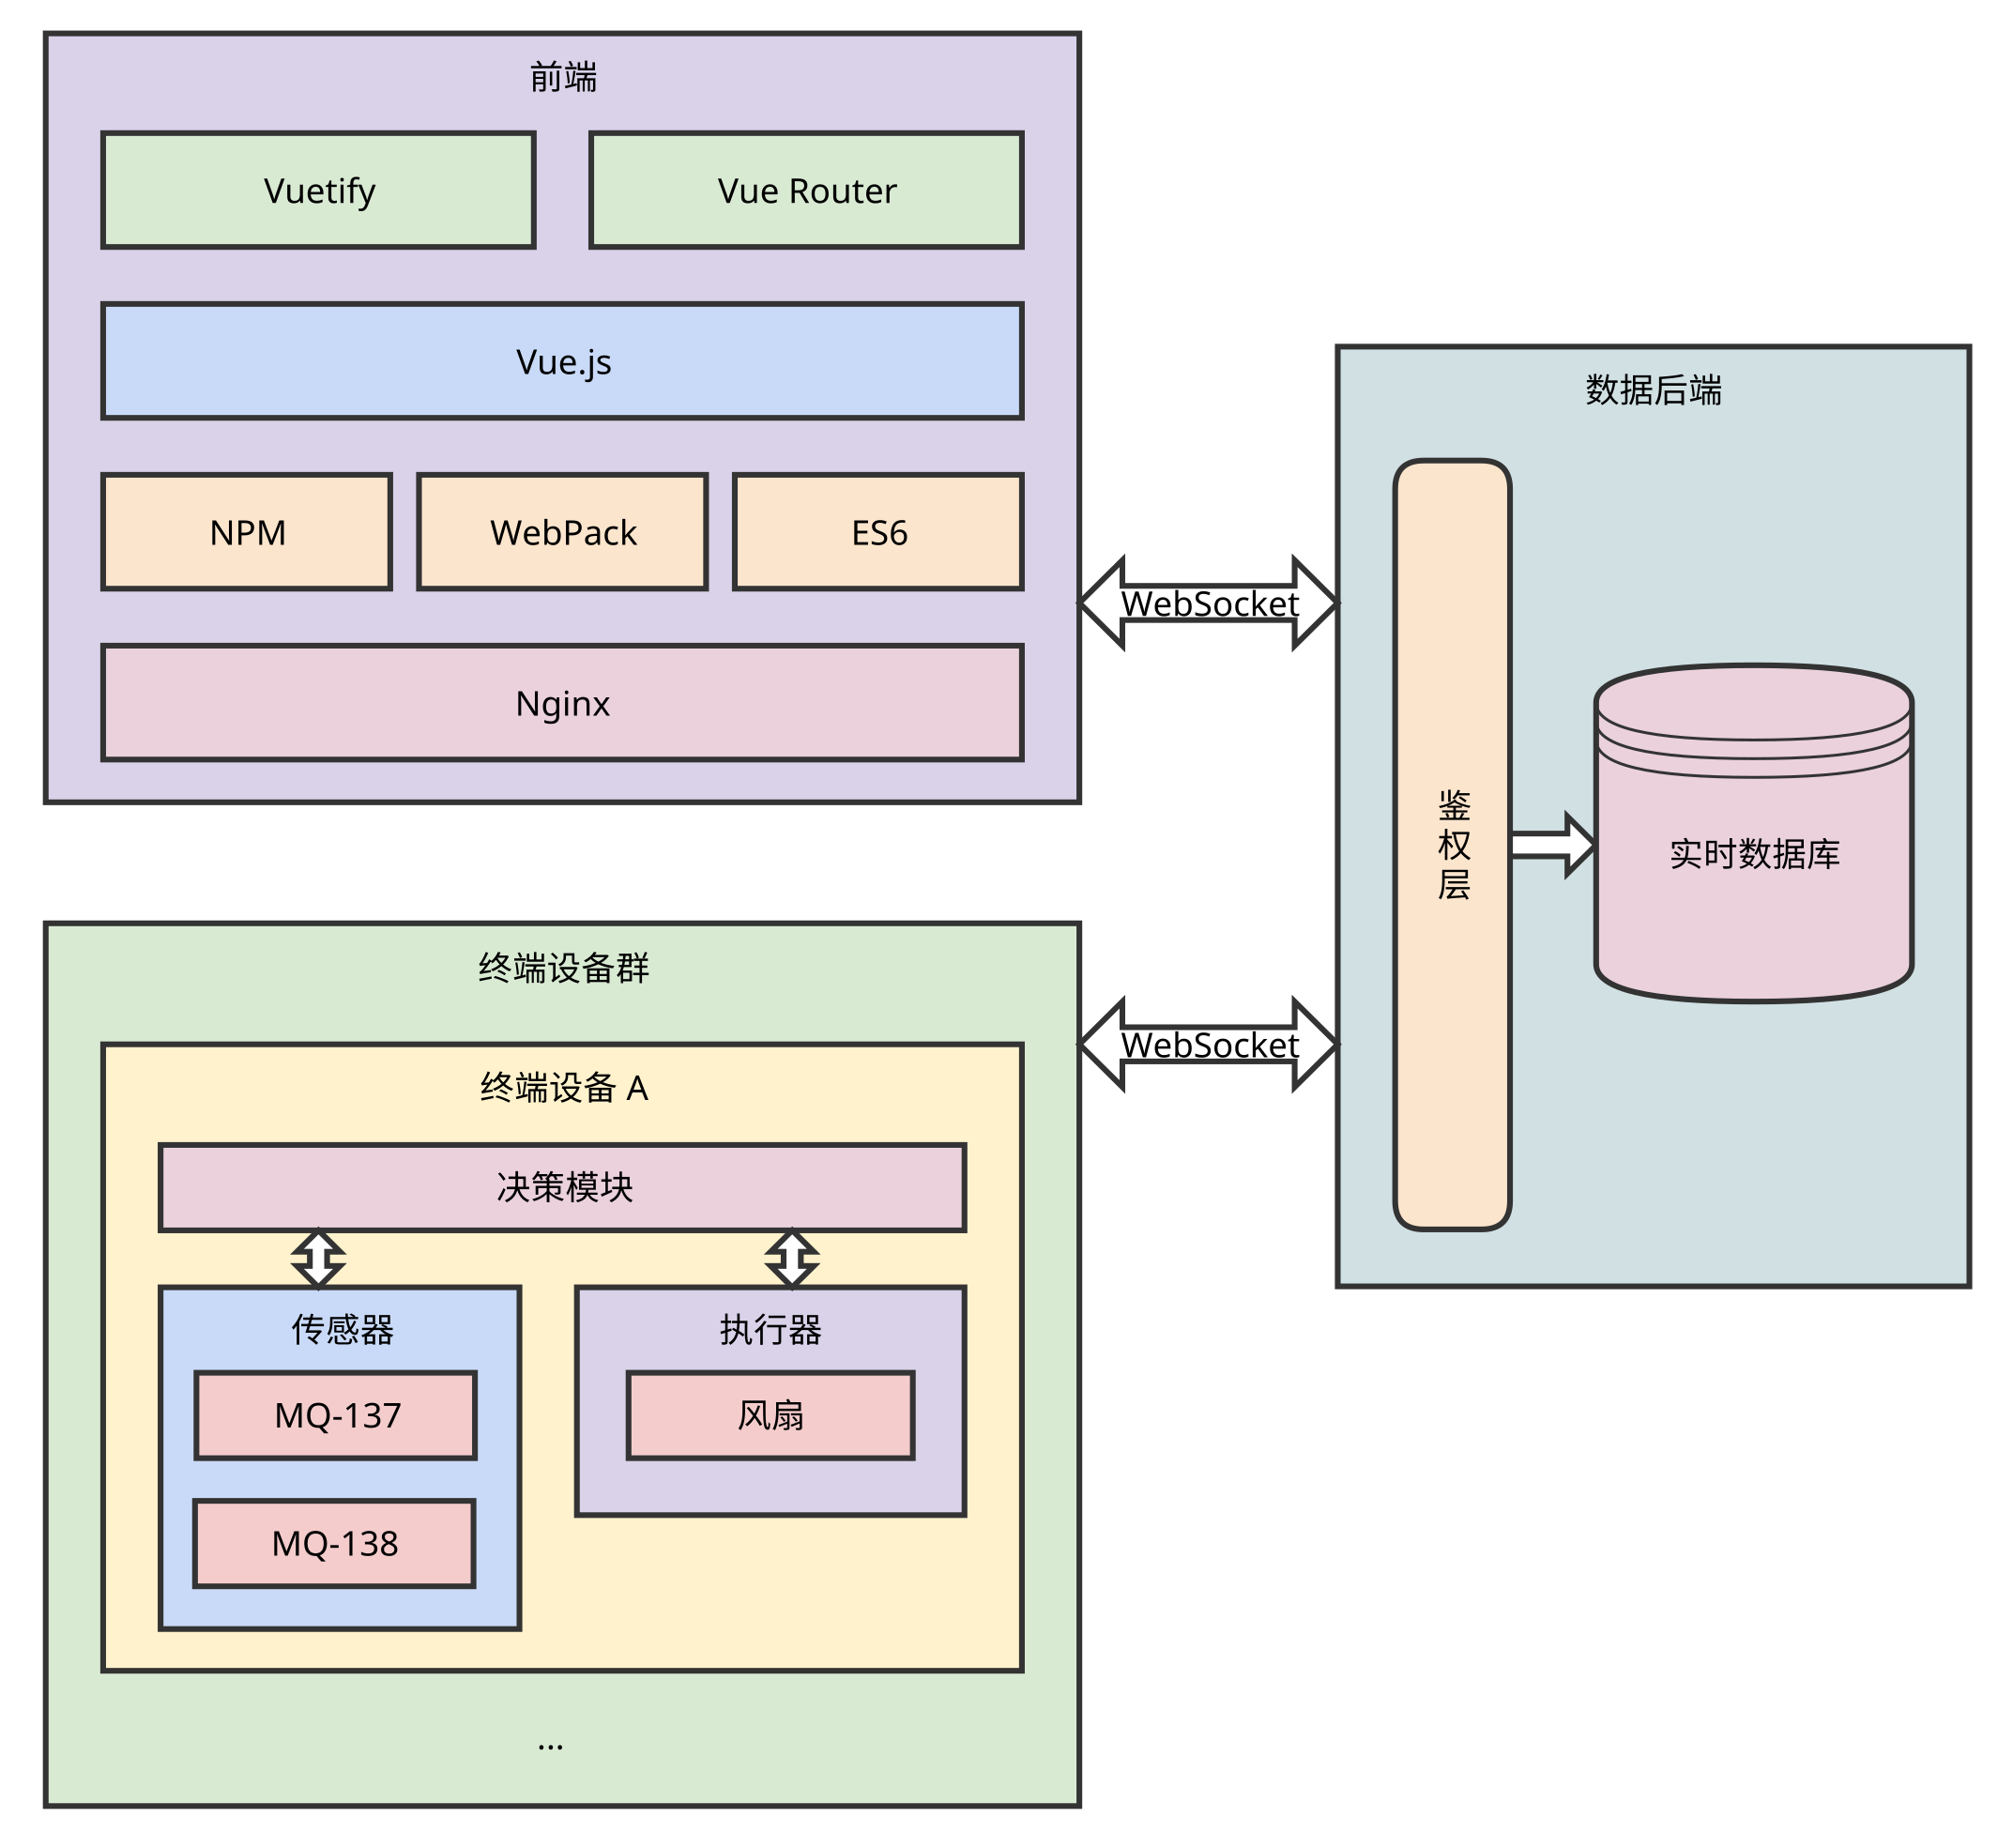
\includegraphics[width=.7\textwidth]{diagram.png}
    }
    \caption{逻辑架构}\label{fig:diagram}
\end{figure}
\subsubsection{技术选型}
终端设备为树莓派开发版,其上搭载 H2S(g) 与 NH3(g) 传感器,以实现对厕所臭味状况的实时感知。同时,可外接继电器或输出其他信号,以实现智能开启排风扇、喷洒除臭剂等主动防控功能。设备使用 5V 3A Type-C USB 供电,原型将使用充电宝/适配器进行供电,在生产环境可以考虑使用热插拔电池包。设备使用 WiFi 或 4G 网络接入互联网,并拥有自己的设备 token,以实时回传数据。

数据后端的存储部分预计由运行在互联网上的本地实时数据库(Couch\-DB, PouchDB 等)服务器或 Serverless 服务(Firebase, LeanCloud 等)实现,以 WebSocket 协议或 Ajax 请求承载 Json API 完成数据的读写。同时,指令以数据的形式写入数据库并在各端间同步,以实现最好的实时性,并便于权限管理。

监控前端为 Web 单页应用,使用 Vuetify UI 框架与 Vue.js 页面框架,展现所有终端记录的臭味浓度图表与除臭运作状态,并在发生异常或除臭手段开始运作时发出警告。同时,使用双向绑定的 MVVM 模型,数据与图表实时刷新,使过去与当前的厕所气味状态和设备运行状态一目了然,便于监控操作。
\subsubsection{系统运行}
在初期,用户需在有检测需求的厕所中安装终端设备。设备可以胶水或螺丝等方式固定在墙上等位置,确保电源联通,并完成网络配置(4G 或 WiFi)。

部署完毕后,用户只需使用任意浏览器打开监控应用,便可一目了然地查看所有厕所的状态,并对紧急状况进行干预。页面上将有一个动态更新的图表,以不同颜色展示各个厕所的状况(气味良好/异常,设备正常/故障,主动除臭是否运行)。当用户指定某一终端,将展示该厕所实时更新的历史气味浓度图表与当前实时变化趋势。用户可在应用中设定主动除臭的气体浓度触发策略以实现自动除臭,或手动强制启动除臭功能以应对突发状况。

如果使用电池供电方案,需要在终端发出电量低警告时及时更换电池。

\section{项目实施计划}
\subsection{项目时间计划}
\subsubsection{项目时间流程}
\textbf{第1周:}确定系统整体框架,初步确定实现方案,购买硬件设备与云端服务\\

\textbf{第2周:}配置RaspberryPi及云端环境,编写后端程序,实现数据存取操作\\

\textbf{第3周:}编写前端程序,实现数据、图表、除臭系统运行状态更新查看功能\\

\textbf{第4周:}完善前端程序,实现后端调控终端除臭系统运行功能\\

\textbf{第5周:}系统整体运行调试,检查、修复漏洞\\

\textbf{第6、7、8周:}美化前端页面,系统长时间运行稳定性测试\\

\subsubsection{项目阶段工作表}
项目阶段工作表见 表 \ref{tab:time}。

\begin{table}[htbp]
	\noindent\makebox[\textwidth]{
		\begin{tabular}{|c|c|c|}
		\hline
			\diagbox{工作阶段}{工作描述}{起止日期}&工作描述&起止日期\\
			\hline
  			第一阶段 & \tabincell{c}{设置项目。 初步确定实施方案。\\进行可行性分析并完成技术选择。制定框架。\\ 购买必要的硬件和云服务。}&10月14日$\sim$ 10月17日\\
			\hline
  			第二阶段 & \tabincell{c}{配置Raspberry Pi和云环境。 \\编写设备端程序并实现数据库数据访问和控制操作。\\ 编写一个前端程序,以实现实时数据,图表,\\除臭系统运行状态的更新和查看功能。} &  10月24日$\sim$ 10月31日\\
			\hline
  			第三阶段 & \tabincell{c}{ 完善前端程序并补充其他辅助功能。\\ 在前端添加/删除设备,使数据库紧凑。 \\若非管理员,则将用户锁定在数据库操作之外。}  &11月25日$\sim$ 11月30日\\
			\hline
  			第四阶段 & \tabincell{c}{实现设备端除臭系统的操作功能。\\ 美化页面,调试系统的整体操作。\\ 对长时间运行的系统进行稳定性测试。}  &  12月2日$\sim$  12月7日 \\
\hline
\end{tabular}
}\caption{项目时间流程}\label{tab:time}
\end{table}

\subsection{经费预算}
经费预算见 表 \ref{tab:bom}。
\begin{table}[htbp]
    \noindent\makebox[\textwidth]{
        \begin{tabular}{c|c|c|c}
            \hline
            材料名称             & 单价/元 & 数量 & 总价/元 \\
            \hline
            Raspberry Pi 4B      & 435     & 1    & 435     \\
            \hline
            MQ-137 氨气传感器    & 85      & 1    & 85      \\
            \hline
            MQ-136 硫化氢传感器  & 85      & 1    & 85      \\
            \hline
            BG0903-B049-P0S 风扇 & 20      & 1    & 20      \\
            \hline
            ADC 模块             & 148     & 1    & 148     \\
            \hline
            腾讯云CVM           & 120     & 1    & 120     \\
            \hline
            总计                 & ---     & ---  & 893     \\
            \hline
        \end{tabular}
    }
    \caption{经费预算}\label{tab:bom}
\end{table}

\section{系统实施方案}
\subsection{成员分工}
本小组成员包括五人,整个项目开展过程采取分工与协作相结合的方式进行。在确定目标、方案设计、终端设备制作过程中,主要以小组合作方式展开工作。在进行设备端程序编写、前端程序编写、购置材料以及调研报告撰写环节,主要以分工的形式落实。小组合作时,小组成员积极参与讨论,就同一问题提出自己的观点,集思广益,发现了较多细节上的问题并找到了相应的改进方法。分工开展设备个人任务时,小组每一个成员发挥自身优势,积极做好个人的工作以实现整体工作的良好推进。总之,每一位小组成员都为项目贡献出了一份自己的力量。
\subsection{系统方案设计}
\subsubsection{整体框架}
本项目具体开发时选择的整体逻辑架构如图 \ref{fig:diagram2} 所示。
\begin{figure}[h]
    \noindent\makebox[\textwidth]{
        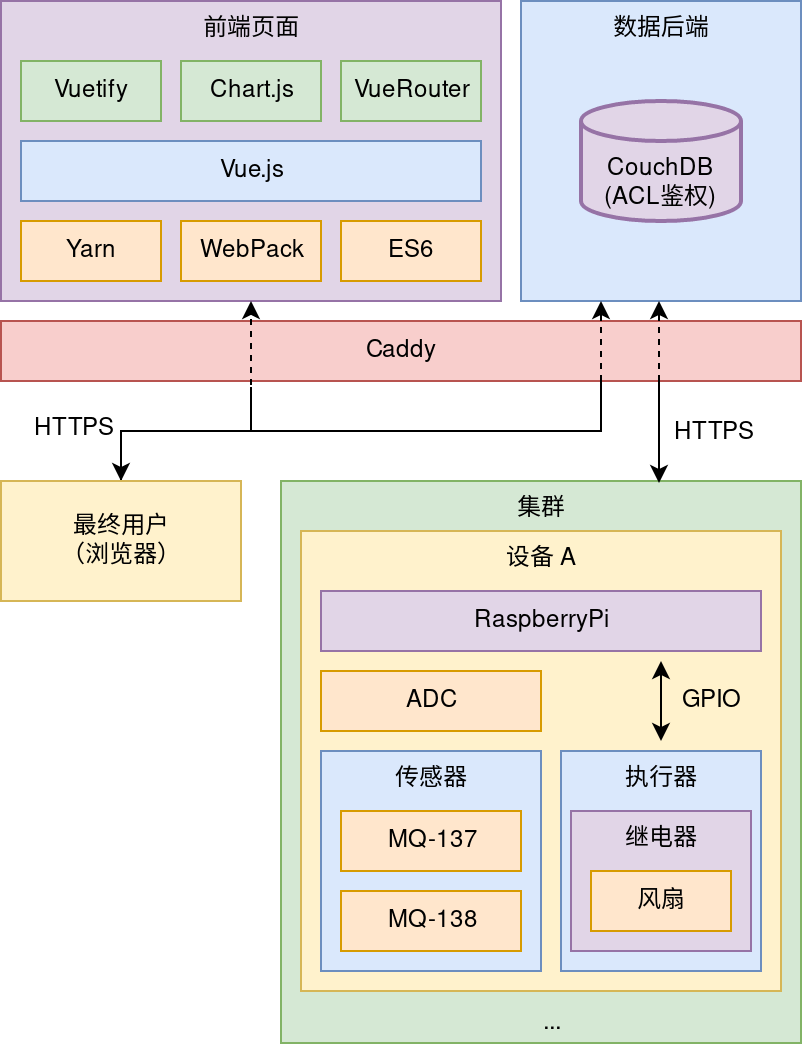
\includegraphics[width=.5\textwidth]{diagram2.png}
    }
    \caption{整体逻辑架构}\label{fig:diagram2}
\end{figure}


\subsubsection{前端系统方案}
监控前端使用 Vuetify UI\footnote{a material component framework for Vue, which is licensed under the MIT License.} 框架与 Vue.js\footnote{the progressive javascript framework, which is licensed under the MIT License.} 页面框架,展现所有终端记录的臭味浓度图表与除臭运作状态。除了可以实时显示当前状态下的臭味浓度数据之外,我们使用了基于时间分类的浓度图标显示方案,可以显示过去一小时/过去三天的臭味浓度曲线图。在自动模式下,若气体臭味浓度超过预设阈值上界,则会通过设备端控制程序向硬件设备发送启动排风扇的指令,当设备反馈的气体臭味浓度下降到预设阈值下界以下时,则会向硬件设备发送启关闭排风扇的指令。在手动模式下,若选择常开,则硬件设备的排风扇会无视气体浓度变化持续保持开启状态,若选择常关,则硬件设备的排风扇会持续保持关闭状态。

\subsubsection{后端系统方案}
数据后端的存储部分由运行在服务器上的实时数据库 CouchDB\footnote{an open-source document-oriented NoSQL database, which is licensed under the Apache License 2.0.} 实现,以 HTTPS协议 承载 Json API 完成数据的读写。权限管理方面我们使用了Couch-DB自带的解决方案。
在我们的设计中,数据库内分为以下几个数据表: SUMMARY 、 DATAGRID 、 \_USER 。对于从硬件系统获取到的气体浓度数据,我们对其添加时间戳后存入 DATAGRID 数据表。 对于设备的添加/删除信息、控制设备的指令以及设备状态数据(在线、离线),我们将其存入 SUMMARY 数据表。对于管理员用户与普通用户的账号与密码,我们将其密码 PBKDF2 处理后存入 \_USER 表,我们也将每个设备分别独立为一个用户,存入 \_USER 表。
在权限设计方案中,我们有以下几类用户:SUDOER , ADMIN , DEVICE。对于 SUDOER 类型的用户,他们有权限删除设备,修改设备工作模式\footnote{即排风扇控制模式,分为自动模式、手动模式:常开、手动模式:常关}。对于 ADMIN 类型的用户,他们完全继承了 SUDOER 的权限,并在这个基础上拥有了添加设备、管理数据库的权限。对于 DEVICE 类型的用户,此类用户隐式地存在于硬件设备中,作为硬件设备对 DATAGRID 数据表进行写入操作的权限提供者。
\subsubsection{硬件系统方案}
硬件设备为树莓派开发版,其上搭载 MQ-136\footnote{MQ-136 Gas Sensor for Hydrogen Sulfide} 与 MQ-137\footnote{MQ-137 Gas Sensor for Ammonia} 传感器,配合 High-Precision AD/DA Board 以实现对厕所臭味状况的实时感知。同时,通过带光耦隔离的继电器以实现控制排风扇的功能。设备使用 5V 3A Type-C USB 供电,演示原型将使用充电宝/适配器进行供电,在生产环境可以考虑使用热插拔电池包。设备使用 WiFi 或 4G 网络接入互联网,并拥有自己的设备用户,以实时回传数据。在数据读取方面,我们通过GPIO与AD/DA芯片通信来读取传感器数据。对于断网的情况,在设备端我们维护了一个本地消息队列,从而保证在设备重新联网后能够将断网期间采集到的数据上传至数据库。


\section{系统功能展示}

\subsection{面向用户的界面}
\subsubsection{设备状态总览}
设备状态总览界面如 图 \ref{fig:device_overall} 所示。在演示版本内,我们部署了1台硬件设备与2台虚拟设备,其中 DEVICE\_305 部署于上海交通大学闵行校区东10号楼305室内,用于模拟真实的厕所环境, DEVICE\_DUMMY 部署于国内服务器上,用于连续生成测试数据来模拟长期运行的情况, DEVICE\_POOR 部署于国外服务器上,用于模拟网络条件不佳的情况。
\begin{figure}[H]
    \noindent\makebox[\textwidth]{
        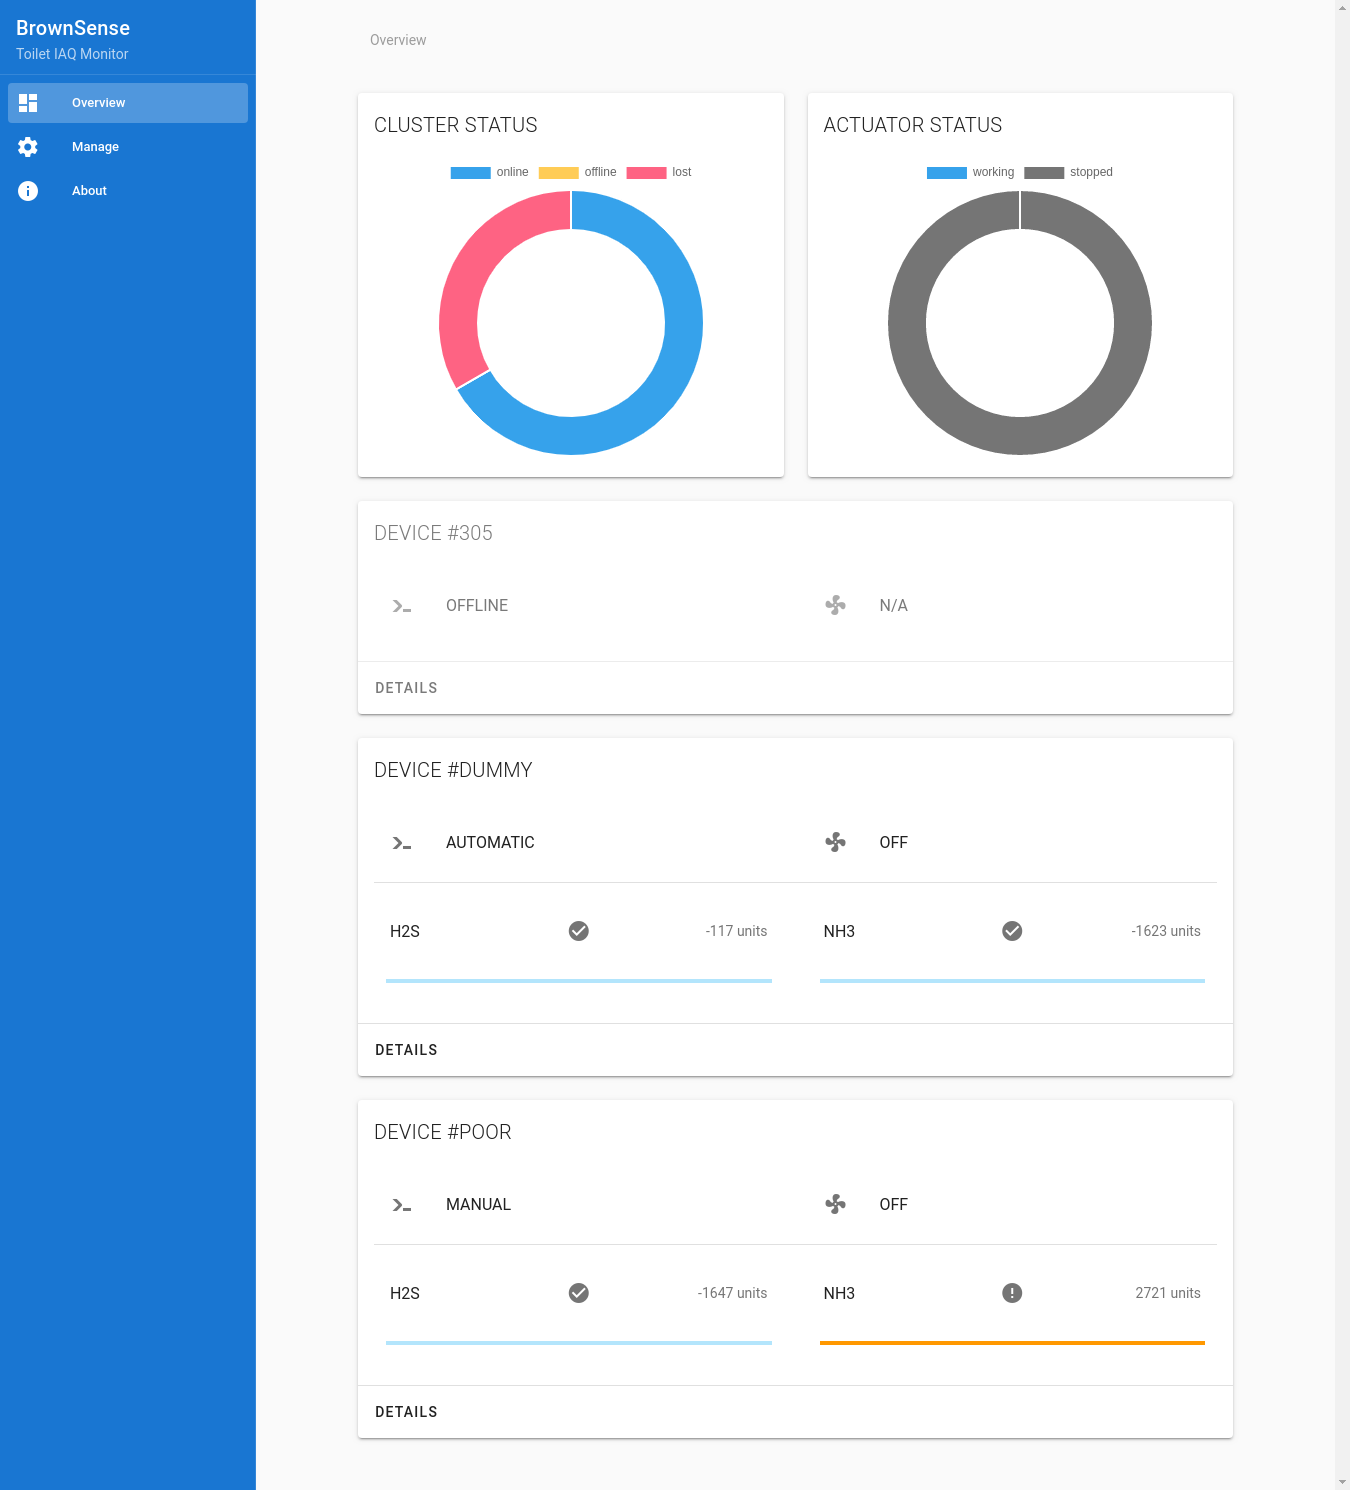
\includegraphics[width=0.9\textwidth]{device_overall.png}
    }
    \caption{设备状态 总览}\label{fig:device_overall}
\end{figure}
\subsubsection{设备详情}
设备详情界面如 图 \ref{fig:device_details} 和 图 \ref{fig:device_details2} 所示。在设备详情总览界面,可以看到实时更新的臭味浓度数据、设备当前工作模式、排风扇运作状态以及迷你图表。在设备详情图表界面,可以通过选择显示过去一小时/过去三天的臭味浓度曲线图。

\begin{figure}[H]
    \noindent\makebox[\textwidth]{
        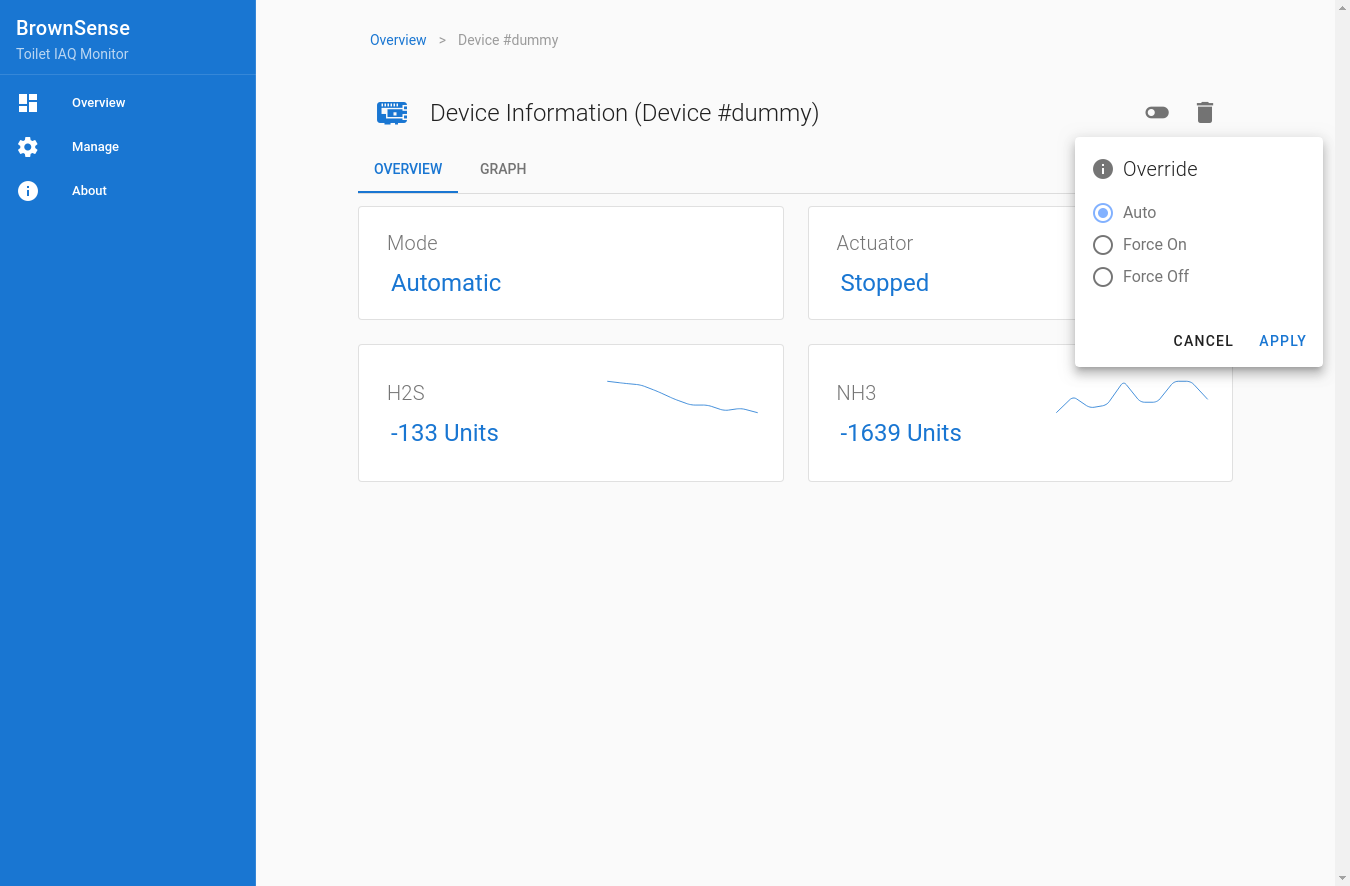
\includegraphics[width=1\textwidth]{device_details.png}
    }
    \caption{设备详情总览}\label{fig:device_details}
\end{figure}
\begin{figure}[H]
    \noindent\makebox[\textwidth]{
        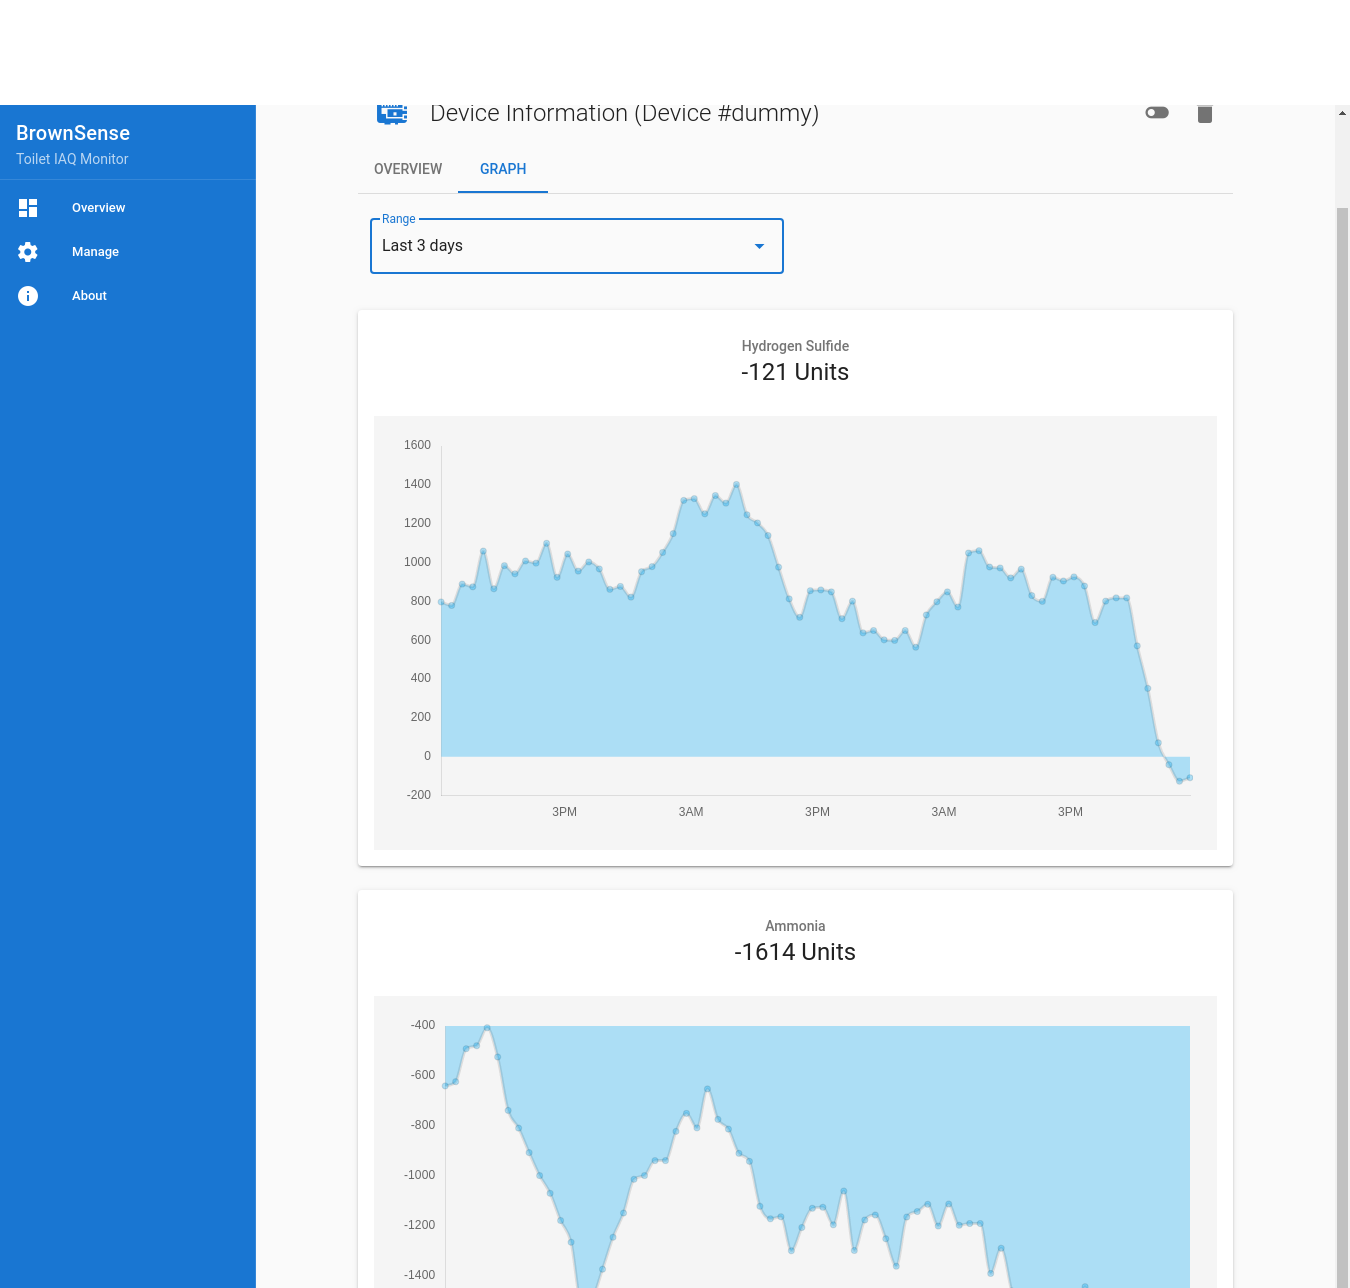
\includegraphics[width=1\textwidth]{device_details2.png}
    }
    \caption{设备详情图表}\label{fig:device_details2}
\end{figure}
\subsubsection{设备管理}
设备管理如 图 \ref{fig:device_details3} 所示。登入拥有 SUDOER 权限的账户后,可以对风扇的工作模式进行切换,并且可以删除对应设备。 

\begin{figure}[H]
    \noindent\makebox[\textwidth]{
        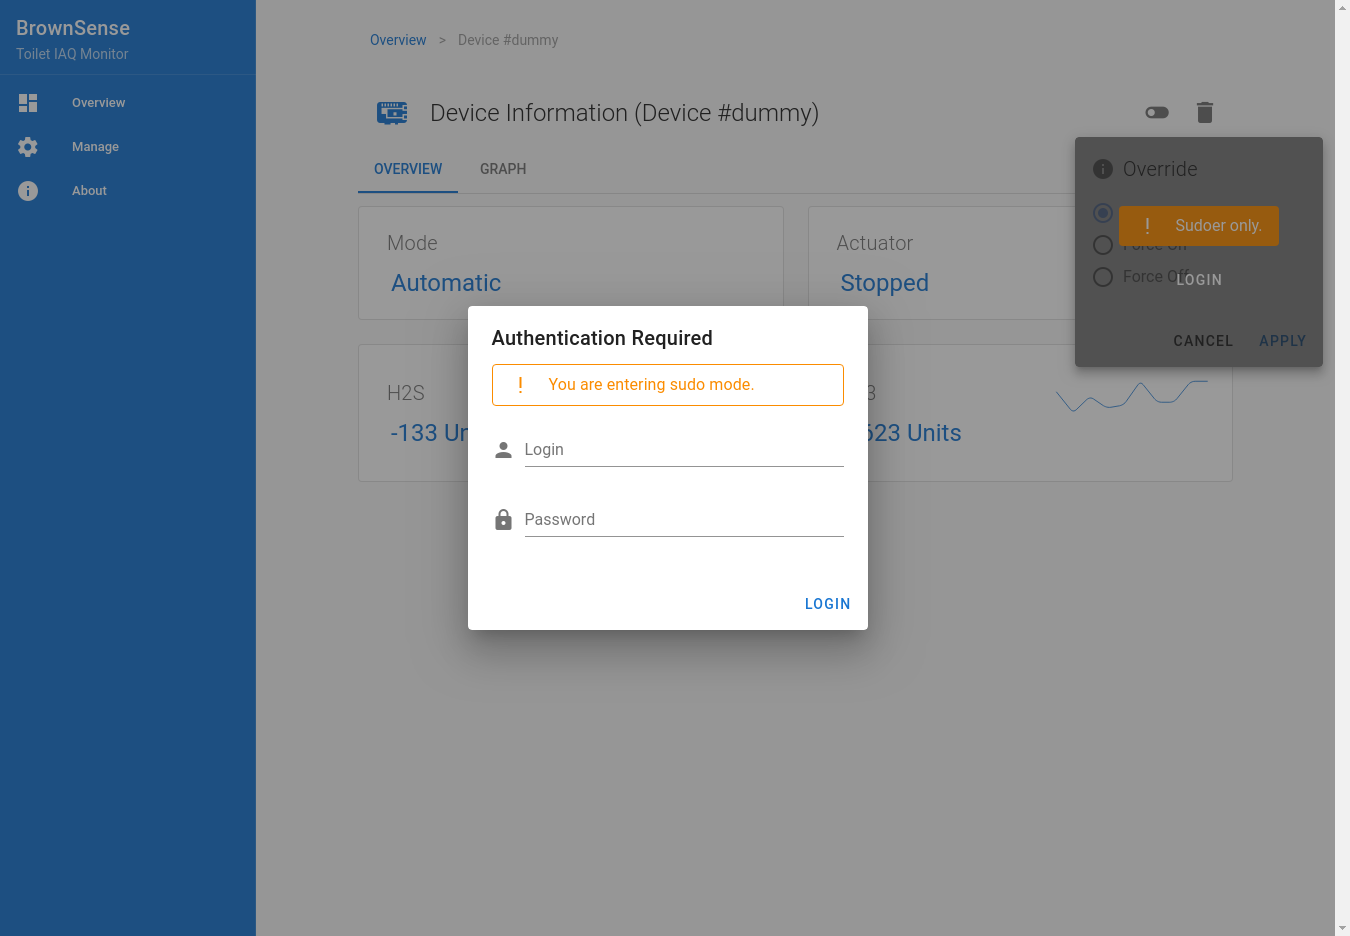
\includegraphics[width=1\textwidth]{device_details3.png}
    }
    \caption{设备管理}\label{fig:device_details3}
\end{figure}

\subsection{面向管理员的界面}
登录拥有 ADMIN 权限的账户后,才可以在管理界面进行后续操作。如 图 \ref{fig:device_admin1} 所示。
\begin{figure}[H]
    \noindent\makebox[\textwidth]{
        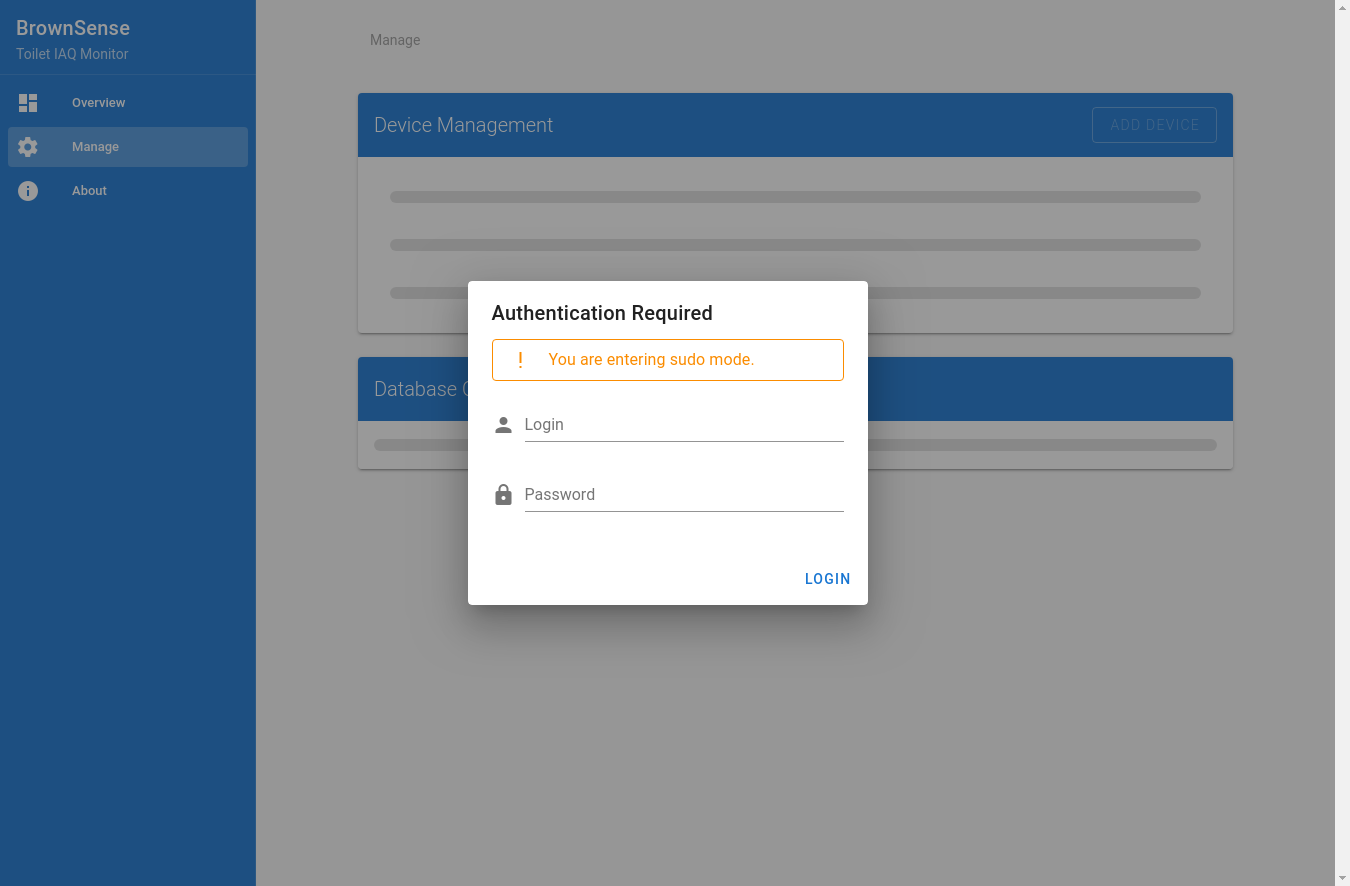
\includegraphics[width=1\textwidth]{device_admin1.png}
    }
    \caption{管理界面}\label{fig:device_admin1}
\end{figure}

\subsubsection{全体设备管理}
如 图 \ref{fig:device_admin2} 所示。在管理界面,可以对所有设备进行删除的操作。并且点击 ADD DEVICE 添加新的设备。
\subsubsection{数据库管理}
如 图 \ref{fig:device_admin2} 所示。在管理界面,可以对数据库进行清理、压缩的操作,通过这样的操作可以保证在系统长期运行、积累大量历史垃圾数据后,仍能恢复如初。

\begin{figure}[H]
    \noindent\makebox[\textwidth]{
        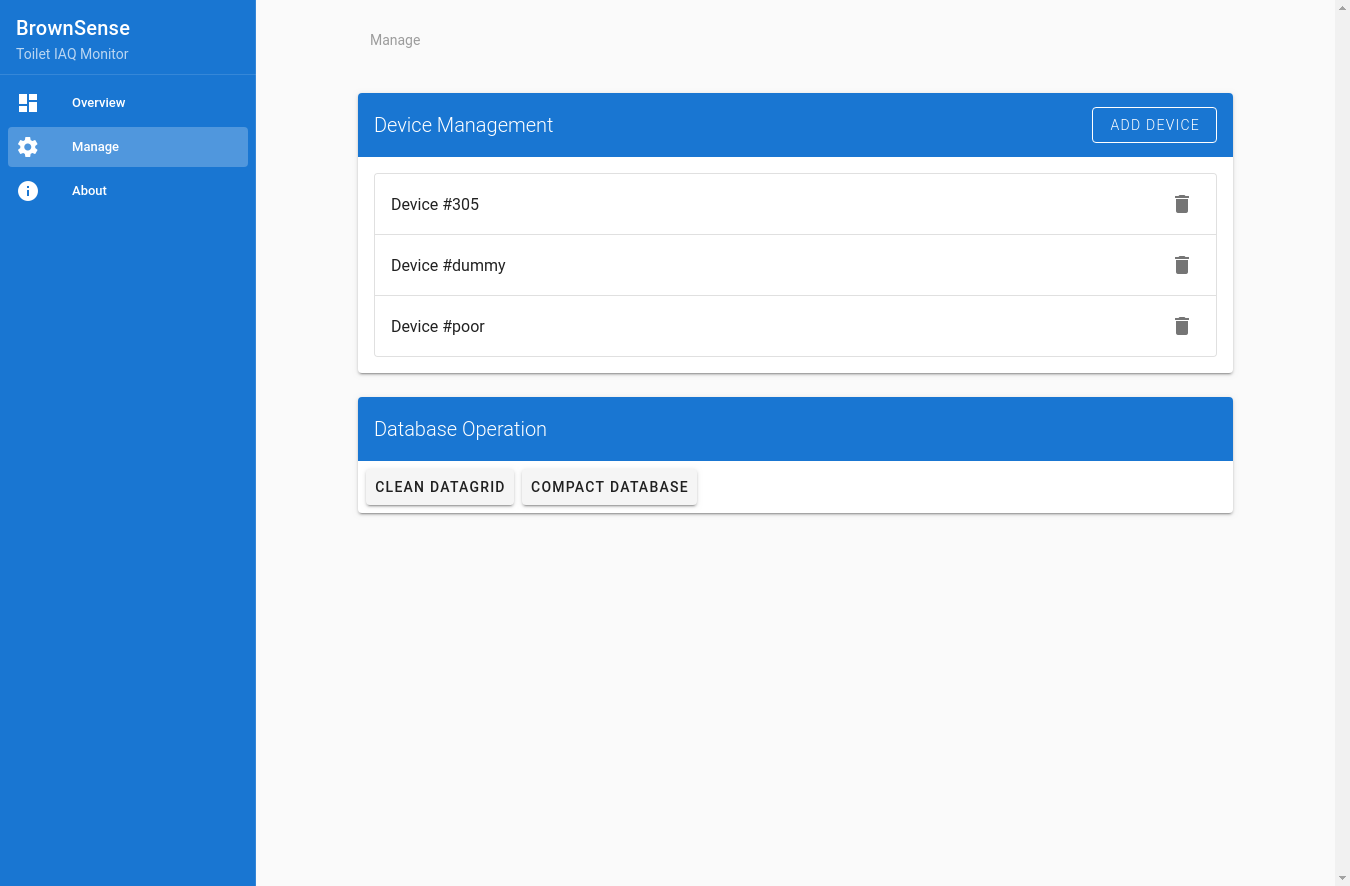
\includegraphics[width=1\textwidth]{device_admin2.png}
    }
    \caption{面向管理员的界面}\label{fig:device_admin2}
\end{figure}

\subsection{硬件功能}
\subsubsection{总览}
如 图 \ref{fig:device} 所示,硬件由四部分组成,分别为 RaspberryPi 、传感器、继电器和排风扇。
\begin{figure}[H]
    \noindent\makebox[\textwidth]{
        \includegraphics[width=1\textwidth]{device.png}
    }
    \caption{硬件总览}\label{fig:device}
\end{figure}
\subsubsection{气体浓度采集}
如图 \ref{fig:device_report} 所示,通过GPIO与AD/DA芯片通信来读取气体传感器数据后,会将它们上传至数据库。
\begin{figure}[H]
    \noindent\makebox[\textwidth]{
        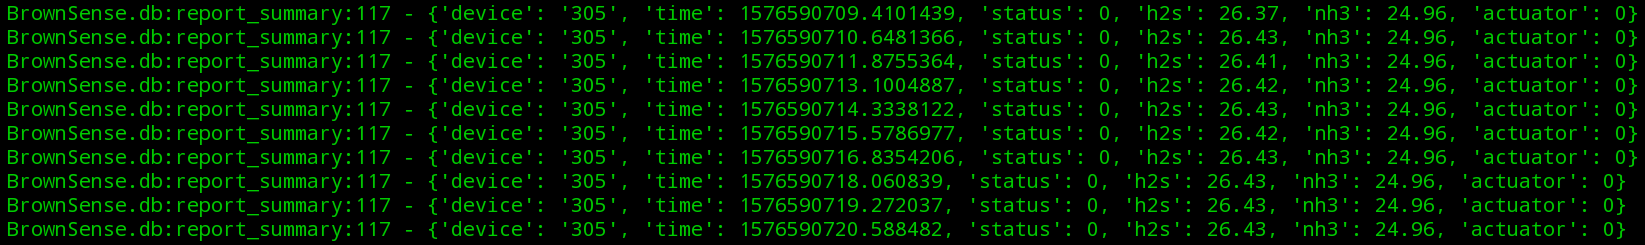
\includegraphics[width=1\textwidth]{device_report.png}
    }
    \caption{气体浓度采集}\label{fig:device_report}
\end{figure}
\subsubsection{排风扇控制}
在自动模式下,若气体臭味浓度超过预设阈值上界,排风扇会保持开启直到气体臭味浓度下降到预设阈值下界以下时,排风扇会保持关闭。在手动模式下,若选择常开,则硬件设备的排风扇会无视气体浓度变化持续保持开启状态,若选择常关,则硬件设备的排风扇会持续保持关闭状态。
排风扇关闭、排风扇开启时状态如 图 \ref{fig:device_onoff} 所示,注意到此时继电器
上红色LED亮起,表面此时继电器闭合,使排风扇开始工作。

\begin{figure}[H]
\centering
\begin{minipage}{0.4\linewidth}

    \noindent\makebox[\textwidth]{
        \includegraphics[width=1.2\textwidth]{device_off.JPG}
    }
	\centerline{(a) 排风扇关闭时}
\end{minipage}
\hfill
\begin{minipage}{0.4\linewidth}

    \noindent\makebox[\textwidth]{
        \includegraphics[width=1.2\textwidth]{device_on.JPG}
    }
	\centerline{(b) 排风扇开启时}
\end{minipage}

\caption{排风扇控制}\label{fig:device_onoff}

\end{figure}


\section{项目总结}
\subsection{对项目前期方案设计的总结}
在建构一种基于RaspberryPi的在线异味监管系统的目标下,我们先通过小组讨论及发放调查问卷获知智能排风系统的需求,依据需求来确定所制作的系统以及终端设备的特征和功能,这就保证了产品研发出来后的市场需求。确定需求后,我组对满足需求的功能进行综合讨论分析,经过集思广益,结合实际情况和经费要求,最终确定了以搭载H2S(g)与NH3(g)传感器的树莓派开发版作为终端设备、以使用 Vuetify UI 框架与 Vue.js 页面框架的Web 单页应用作为监控前端、由运行在互联网上的本地实时数据库(CouchDB, PouchDB 等)服务器作为数据后端的存储部分并以 HTTPS 协议完成读写数据的方案,该过程保证了项目的高效可行。

\subsection{对项目产品的评价}
此套系统可适用于大规模的厕所臭味情况监控与除臭管理,为现实生活中需要大规模管理厕所的情况提供了智能的解决方案,在很大程度上降低了大规模(公共)厕所维护的人力成本。本系统在开发时将核心代码进行了深度封装,为在现实生活中的部署提供了很大的便利。在实际使用过程中,产品也实现了我们所需要的各种功能,如定量检测空气污染物浓度、实时反馈空气质量、排风系统的自动开关和手动开关等等,项目效果较好。当然,产品的长期使用要求对数据后端和在线系统进行人工定期维护,对产品的使用产生了一定的限制。

\subsection{对生产效率的评价}
本项目预期在本学期内完成。在经过详细的初步方案设计后,小组成员很快购买了硬件,并开始了程序的编写和调试。在学期第12周左右项目基本完工,留下了较充裕的时间来调试和改进产品。小组成员充分发挥团队协作精神,项目完成效率很高。

\subsection{对实施项目的经验总结}
最初方案中,设计数据的读写预想以Websocket协议或Ajax请求承载Json API完成数据的读写,后因为条件的限制最终采用了 HTTPS 协议。较早地发现问题帮助我们很快寻找到了解决方案。此外,一些初步没有考虑到的问题,如用户界面的外观,以及管理员权限的分级,数据的保存和清楚等都在后期调试和试用的时候显现了出来,并得到了我们及时的改进和优化,这也充分体现组员和其他试用者对产品完善的重要性。

\subsection{前景展望}
受开发成本等因素的限制,我们在演示版本上使用的气体传感器并不是精准的电化学传感器,根据我们从传感器产品手册上的传感器特性图 (图\ref{PIC:MINI}),由于我们的目标浓度区间在100ppm以下,由于该曲线突变过于剧烈,以目前的条件我们无法得到以ppm为单位的浓度数据。在演示版本,我们对原始数据进行线性映射来模拟真实的浓度数据。若能通过标准试剂对传感器进行更为精确的特性测量,就能得到以ppm为单位的真实浓度数据。
\begin{figure}[H]
\centering
\begin{minipage}{0.4\linewidth}

    \noindent\makebox[\textwidth]{
        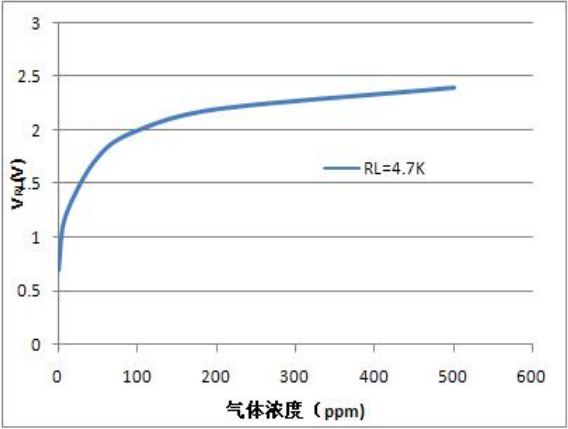
\includegraphics[width=1.2\textwidth]{mq136.png}
    }
	\centerline{(a) MQ136}
\end{minipage}
\hfill
\begin{minipage}{0.4\linewidth}

    \noindent\makebox[\textwidth]{
        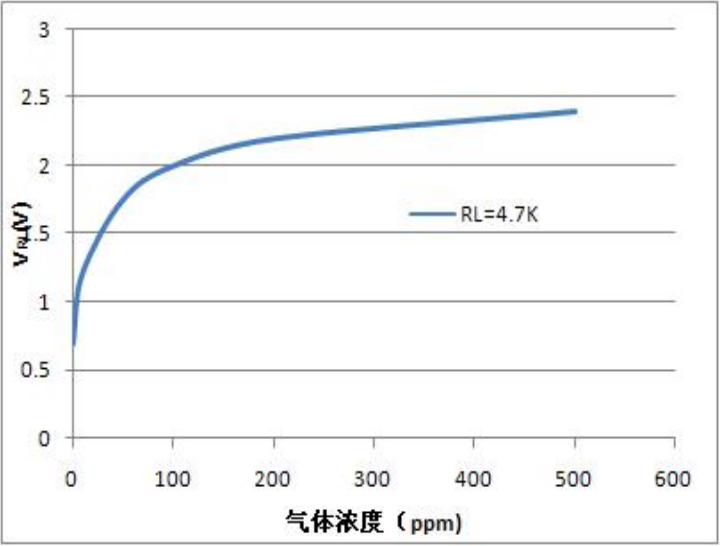
\includegraphics[width=1.2\textwidth]{mq137.png}
    }
	\centerline{(b) MQ137}
\end{minipage}

\caption{传感器特性图}\label{PIC:MINI}

\end{figure}

\newpage
\section*{致谢}
\addcontentsline{toc}{section}{致谢}
本次项目完成顺利,最终产品满足预期要求,整个过程得到了多方帮助。首先要感谢的是学校对本项目的资金支持以及设备支持。感谢老师的指导,助教的帮助,组长及组员对本次项目的热情付出。感谢其他直接或间接对本次项目做出贡献的人,在此表示衷心感谢。

\begin{appendix}
\section{附录}
\subsection{系统全套代码}
见本系统的开源地址 : \url{https://github.com/PhotonQuantum/BrownSense}
\end{appendix}

\pagebreak
\end{document}